\section{Action-editing observations and motivation}
\label{sec:unified-observations}
Action-editing failures and generation--editing comparisons motivate
learning from a model's own text-to-video demonstrations. We examine these
observations and the temporal evidence for such action anchors.

\subsection{Action editing in closed video models}
\label{sec:commercial-editor-probes}
Four archived cases from Gemini Omni Flash~\citep{google2026geminiomni}
and Kling Omni~\citep{kling2025omni} probe timing, substitution,
interactions, and event outcomes. The archive records model names but not
exact revisions or seeds; these examples illustrate failure modes without
estimating their prevalence.

\begin{figure}[!htbp]
 \centering
 \includegraphics[width=\linewidth]{omni_action_timing.pdf}
 \caption{\textbf{Temporal behavior in action-editing probes.}
 (a) Under the same instruction, Gemini Omni Flash retains the raised-leg
 pose through 4.0\,s and lowers the leg near the end; Kling Omni retains the
 pose in the shown sequence.
 (b) Gemini Omni Flash retains the walk toward the door before adding
 drinking. The source in (b) is generated, and its instruction is translated
 from the archived filename. Frames are uncropped; timestamps start at
 each video's first decoded frame and do not imply event alignment.}
 \label{fig:omni-action-timing}
\end{figure}

\paragraph{Source motion can survive the edit.}
Figure~\ref{fig:omni-action-timing}(a) separates reaching a requested
endpoint from changing the preceding trajectory: Gemini Omni Flash
lowers the leg only near the end, whereas Kling Omni retains the raised
pose. The instruction sets no exact onset, so timing is reported directly.
In (b), ``instead'' explicitly requires replacing the walk; drinking is
added after the walk survives. The presence of the target action alone
therefore does not establish successful temporal substitution.

\begin{figure}[!htbp]
 \centering
 \includegraphics[width=\linewidth]{omni_action_and_preservation.pdf}
 \caption{\textbf{Interaction and outcome edits with Gemini Omni Flash.}
 (a) Eyebrow makeup is achieved, but Edit A also shifts the rendered skin
 tone; Edit B changes the mirror-surface color alongside the requested
 subject change.
 (b) Edit A does not clearly show the requested post-and-wide outcome;
 Edit B changes event timing and introduces camera cuts.
 A and B are independent edits of the same source in each panel.
 Instructions reproduce the full archived edit text; for soccer, the
 archive contains only the changed sentences.
 Frames are uncropped and follow Figure~\ref{fig:omni-action-timing}'s
 time convention.}
 \label{fig:omni-action-preservation}
\end{figure}

\paragraph{Action changes can alter unrelated appearance.}
In Figure~\ref{fig:omni-action-preservation}(a), Edit A redirects the tool
to the eyebrows but subtly changes the woman's rendered skin tone.
Edit B realizes both requested changes, while the mirror surface changes
from blue to brown. These unrequested changes violate the non-target
preservation required for atomic action editing and modular composition
of subject and action edits.

\paragraph{Event outcomes and continuity can remain uncontrolled.}
In Figure~\ref{fig:omni-action-preservation}(b), Edit A preserves much of
the source without a clear post-and-wide outcome. Edit B brings the shot
forward and replaces the continuous tracking sequence with reaction
shots and a wide view. These cases motivate separate evaluation of action
execution, temporal structure, and non-target preservation.

\subsection{A generation--editing gap within unified models}
\label{subsec:unified-generation-gap}
To examine whether editing failures reflect a lack of action knowledge,
we compare generation and editing in OmniVideo2-A14B~\citep{yang2026omnivideo2}
and Bernini-R (14B)~\citep{bernini2026planning}.
Figure~\ref{fig:unified-generation-editing} extends the main-text
comparison with three additional cases.

\begin{figure}[!htbp]
 \centering
 \includegraphics[width=\linewidth]{unified_generation_editing.pdf}
 \caption{\textbf{Additional generation--editing comparisons in unified video models.}
 (a) Lifting a barbell from the floor to the waist; (b) rubbing the eyes and
 covering the face with both hands; (c) clapping instead of bowing.
 Each panel shows the source and real target above video editing (left)
 and text-to-video generation (right), with OmniVideo2-A14B and Bernini-R
 (14B) in the two model rows. Instructions specify the requested action
 changes; chronological frames are sampled at matching positions.}
 \label{fig:unified-generation-editing}
\end{figure}

\paragraph{Comparison protocol.}
Both models and modes use the same target-action description and static
context for each case, with a common seed, 81 frames, 25 fps, and 40 sampling
steps. Native conditioning and guidance settings are retained. Only editing
receives the source video; real targets are visual references, not inference
inputs. We show frames 1, 28, 54, and 81 without cropping or changing aspect ratios.

\paragraph{Generation competence does not ensure editing competence.}
An edit can retain source motion or alter appearance even when generation
follows the action more faithfully. In the eye-rubbing case, a raised source
arm persists in an edit, whereas generation depicts rubbing followed by a
two-hand face cover. Useful action knowledge is available in generation
but not effectively expressed in editing. This comparison concerns action
following; T2V has no source-preservation requirement.

\subsection{Recovering action capability through self-generated demonstrations}
\label{subsec:self-evolving-motivation}
\begin{wrapfigure}{r}{0.54\textwidth}
 \centering
 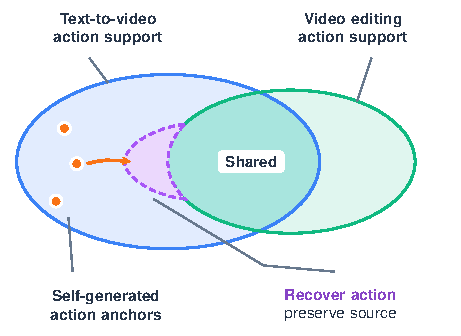
\includegraphics[width=\linewidth]{action_support_recovery.pdf}
 \caption{\textbf{Conceptual view of action recovery.}
 Self-generated anchors (orange) guide recovery of action modes missing
 from the editor (purple), subject to source preservation. Areas are illustrative.}
 \label{fig:action-support-recovery}
\end{wrapfigure}
The gap suggests a potential limitation of generation-to-editing adaptation:
action capability available under text conditioning may be less accessible
when the model must also condition on a source video. Source conditioning
provides the appearance to preserve, but also exposes the model to the
motion that should change. The observed source-action persistence is
consistent with this constraint on expressing the requested action.
It does not by itself establish that adaptation erased the underlying
capability, since the same unified model can still express it in generation.

Figure~\ref{fig:action-support-recovery} illustrates our recovery objective.
The blue and green regions represent action capabilities accessible in
text-to-video generation and source-conditioned editing, respectively.
Their mismatch motivates using self-generated videos as action evidence
for the editor. The desired recovery, shown in purple, must realize the
target action with the source's identity and scene. A generated video is
therefore an action demonstration, not a paired editing target whose
appearance should be copied.

This provides a route to \emph{self-evolving} action editing. The model
first generates demonstrations of the requested action in text-to-video
mode. VADD isolates their dynamics into action anchors and uses those
anchors to guide source-conditioned editing. The model's own generation
capability can thereby supply supervision for improving its editing
capability, without requiring a target video with matching source content.
Repeating demonstration generation and editor refinement is a natural
extension of this mechanism; the observations here motivate that loop
rather than establish gains from repeated iterations.

\subsection{Temporal evidence for self-generated action anchors}
\label{subsec:anchor-temporal-evidence}
We further examine whether self-generated videos carry stronger target-action
evidence than edited outputs in a separate audit of 128 source--target event
pairs. This audit uses a frozen Bernini-R \emph{1.3B} checkpoint, distinct
from the 14B model in Figure~\ref{fig:unified-generation-editing}.
Each pair yields one text-to-video sample and one source-conditioned edit,
using the same target description and seed, 81 frames, 25 fps, and 40 sampling
steps. The real target is used only for evaluation. Manual review prefers
the generated action demonstration in 114 pairs and the edited output in 12,
and records two ties.

\paragraph{A descriptor that retains temporal order.}
We use frozen V-JEPA2 ViT-L features~\citep{assran2025vjepa2}. Each video is sampled into 64 frames,
center-cropped and resized to $256\!\times\!256$ for feature extraction.
Spatial pooling yields 32 ordered vectors of dimension 1,024.
We subtract their temporal mean, concatenate the centered sequence and
its directed differences at strides 1, 2, and 4 in temporal order, and
$\ell_2$-normalize the result, denoted by $\psi_{\mathrm{ord}}(V)$.
Centering removes the temporally constant component of the feature
sequence, while directed differences retain changes and their ordering;
this construction does not assume perfect appearance invariance.

\paragraph{Target action relative to source motion.}
For a candidate video $V$, a real target $V_{\mathrm{tar}}$, and a source
$V_{\mathrm{s}}$, we compute
\begin{equation}
 m_{\mathrm{act}}(V)=
 \cos\!\left(\psi_{\mathrm{ord}}(V),\psi_{\mathrm{ord}}(V_{\mathrm{tar}})\right)
 -\cos\!\left(\psi_{\mathrm{ord}}(V),\psi_{\mathrm{ord}}(V_{\mathrm{s}})\right).
 \label{eq:anchor-action-margin}
\end{equation}
This margin compares evidence of the target trajectory against source
motion. It measures video--video similarity to action references, not
direct video--text similarity to the instruction. To avoid identical-frame
self-comparisons, target and source references use the one-quarter position
of each of 64 temporal bins; candidates and controls use the three-quarter
position. A higher margin is preferred, with differences within $0.005$
treated as ties.

\begin{table}[!htbp]
 \centering
 \caption{\textbf{Temporal controls on the 128-pair audit.}
 Counts indicate that the forward real target scores more than $0.005$
 above each control. A descriptor qualifies for candidate comparison only
 if all three counts reach at least 96/128 (75\%). VideoPrism uses a target-text
 minus source-text cosine margin; both V-JEPA2 descriptors use
 Equation~\ref{eq:anchor-action-margin} with their respective features.}
 \label{tab:anchor-temporal-controls}
 \small
 \renewcommand{\arraystretch}{1.12}
 \setlength{\tabcolsep}{7.5pt}
 \begin{tabular}{@{}lcccc@{}}
 \toprule
 Descriptor & Source & Reversed target & Shuffled target & Qualifies \\
 \midrule
 VideoPrism text margin & 90/128 & 0/128 & 5/128 & No \\
 V-JEPA2 global mean & 128/128 & 98/128 & 21/128 & No \\
 V-JEPA2 ordered residual & 128/128 & 128/128 & 121/128 & Yes \\
 \bottomrule
 \end{tabular}
\end{table}

\paragraph{Checking sensitivity to source motion and temporal order.}
Before comparing candidates, we test whether the descriptor distinguishes
the forward real target from the unchanged source, a reversed target, and
a target with three temporal segments shuffled.
Table~\ref{tab:anchor-temporal-controls} shows that the ordered V-JEPA2
descriptor passes the source and reversal controls on all 128 pairs and the
shuffle control on 121. Temporal mean pooling fails the shuffle control
(21/128), and VideoPrism-LvT-B~\citep{zhao2024videoprism} text margins fail
both order controls (0/128 and 5/128) and fall below the threshold on the
source control (90/128). These comparisons show why a global
similarity score alone is insufficient for the action substitutions studied here.

\begin{table}[!htbp]
 \centering
 \caption{\textbf{Self-generated demonstrations versus edited outputs.}
 Results are from the same 128-pair audit used to qualify the descriptor.
 Mean margins use
 ordered V-JEPA2 features; pairwise preferences use the $0.005$ threshold.}
 \label{tab:anchor-generation-editing-gap}
 \small
 \renewcommand{\arraystretch}{1.12}
 \setlength{\tabcolsep}{9pt}
 \begin{tabular}{@{}lrrr@{}}
 \toprule
 Candidate & Mean $m_{\mathrm{act}}$ & Metric preferred & Human preferred \\
 \midrule
 Self-generated T2V & $-0.01031$ & 125/128 & 114/128 \\
 Source-conditioned edit & $-0.14660$ & 3/128 & 12/128 \\
 Tie & --- & 0/128 & 2/128 \\
 \bottomrule
 \end{tabular}
\end{table}

\paragraph{Evidence for learning from the model's own generation.}
As shown in Table~\ref{tab:anchor-generation-editing-gap}, the mean action
margin is $-0.01031$ for self-generated demonstrations and $-0.14660$ for
edited outputs, a difference of $+0.13629$. The metric prefers the
self-generated demonstration in 125 pairs and the edited output in 3,
with no ties; manual review gives 114, 12, and 2, respectively.
Together with the qualitative examples,
this supports using self-generated T2V videos as target-action evidence
for editing. The margins are relative, so negative means do not establish
absolute action success or failure. The same pairs were used to qualify
the descriptor; the result supports the observed gap on this set, while
held-out evaluation and repeated self-evolution remain to be tested.
